\documentclass[12pt,a4paper]{article}

\usepackage[utf8]{inputenc}
\usepackage{geometry}
\usepackage{graphicx}
\usepackage{xcolor}
\usepackage{booktabs}
\usepackage{longtable}
\usepackage{array}
\usepackage{enumitem}
\usepackage{hyperref}
\usepackage{float}
\usepackage{listings}
\usepackage{caption}

\geometry{left=3cm,right=2.5cm,top=2.5cm,bottom=2.5cm}
\hypersetup{
    colorlinks=true,
    linkcolor=blue,
    urlcolor=blue,
    citecolor=blue
}

\definecolor{codegray}{RGB}{245,247,250}
\definecolor{codetext}{RGB}{31,41,55}
\lstdefinestyle{reportcode}{
    backgroundcolor=\color{codegray},
    basicstyle=\ttfamily\small\color{codetext},
    breaklines=true,
    frame=single,
    framerule=0.3pt,
    rulecolor=\color{gray},
    columns=fullflexible,
    keepspaces=true
}
\lstset{style=reportcode}

\newcommand{\codepath}[1]{\texttt{#1}}

\begin{document}

\begin{titlepage}
\centering
{\Large Posts and Telecommunications Institute of Technology\par}
\vspace{0.5cm}
{\large Faculty of Information Technology 1\par}
\vspace{2cm}
{\LARGE\bfseries Software Architecture and Design Essay\par}
\vspace{0.5cm}
{\Large Building an E-Commerce System Using Microservices and AI\par}
\vfill
\begin{tabular}{rl}
Lecturer: & Tran Dinh Que\\
Student: & B22DCCN441 - Nguyen Duc Khai\\
Class: & E22CNPM01\\
Date: & 2026\\
\end{tabular}
\vfill
\end{titlepage}

\tableofcontents
\newpage
\listoffigures
\listoftables
\newpage

\section{From Monolithic Architecture to Microservices and DDD}

\subsection{Introduction to Monolithic Architecture}

\subsubsection{Concept}

Monolithic Architecture is an architectural style in which the presentation layer, business logic, and data access layer are packaged and deployed as a single application. In a simple e-commerce system, user management, product catalog, cart, order, payment, shipping, and recommendation logic may all be located in the same Django project and connected to the same database.

\subsubsection{Typical Structure}

A typical monolithic application contains three internal layers:

\begin{itemize}
    \item \textbf{Presentation layer}: web pages, forms, templates, or frontend screens.
    \item \textbf{Business logic layer}: product rules, order calculation, payment flow, shipping status, and recommendation logic.
    \item \textbf{Data access layer}: database models, queries, repositories, and migrations.
\end{itemize}

The layers may be internally organized, but they are still deployed as one runtime unit.

\subsubsection{Practical E-Commerce Example}

For an e-commerce system, a monolithic Django application may include:

\begin{itemize}
    \item Product and category management.
    \item User registration, authentication, and role management.
    \item Cart and checkout.
    \item Order history.
    \item Payment and shipping status.
    \item Product recommendation and chatbot modules.
\end{itemize}

This is convenient for a small MVP because development and deployment are simple. However, the architecture becomes difficult to maintain as the domain grows.

\subsubsection{Detailed Drawbacks}

\begin{itemize}
    \item \textbf{Hard to scale}: the whole application must be scaled even if only catalog browsing is under heavy load.
    \item \textbf{High coupling}: a change in payment logic can affect unrelated product or order modules.
    \item \textbf{Risky deployment}: one small bug can break the whole system.
    \item \textbf{Difficult team development}: many developers modify the same codebase and database schema.
    \item \textbf{Weak domain boundaries}: technical folders may hide business dependencies.
\end{itemize}

\subsubsection{When to Use Monolithic Architecture}

Monolithic architecture is still useful when the project is small, the team is small, requirements are not stable, and the main goal is to validate the idea quickly. For a teaching demo, it is useful as a starting point for explaining why microservices and DDD become important.

\subsection{Microservices Architecture}

\subsubsection{Concept}

Microservices Architecture decomposes a system into small, independently deployable services. Each service owns one business capability and communicates with other services through explicit APIs such as REST or gRPC.

\subsubsection{Characteristics}

\begin{itemize}
    \item Each service has its own codebase and deployment unit.
    \item Each service owns its data and avoids direct access to another service's database.
    \item Services communicate through APIs.
    \item Services can be developed, tested, scaled, and deployed independently.
    \item Failures can be isolated more clearly than in a monolith.
\end{itemize}

\subsubsection{Monolithic vs Microservices}

\begin{table}[H]
\centering
\caption{Comparison between monolithic and microservices architecture.}
\label{tab:mono-vs-micro}
\begin{tabular}{p{0.25\linewidth}p{0.32\linewidth}p{0.32\linewidth}}
\toprule
\textbf{Criteria} & \textbf{Monolithic} & \textbf{Microservices}\\
\midrule
Deployment & One application package & Many independently deployed services\\
Database & Usually one shared database & Database-per-service principle\\
Scaling & Scale the whole application & Scale each service independently\\
Development & Simple early development & Better for multiple teams and large domains\\
Failure impact & One module can affect the whole runtime & Failure can be isolated by service boundary\\
Complexity & Lower operational complexity & Higher distributed-system complexity\\
\bottomrule
\end{tabular}
\end{table}

\subsubsection{Advantages}

\begin{itemize}
    \item Independent scaling and deployment.
    \item Clearer business ownership.
    \item Easier technology evolution per service.
    \item Better fault isolation.
    \item Better fit for large systems and team-based development.
\end{itemize}

\subsubsection{Disadvantages}

\begin{itemize}
    \item Network calls add latency and failure cases.
    \item Data consistency becomes harder.
    \item Deployment and monitoring are more complex.
    \item Debugging distributed workflows requires better logs and tracing.
    \item Service boundaries must be designed carefully.
\end{itemize}

\subsubsection{Design Principles}

Good microservice design follows high cohesion, loose coupling, database ownership, API contracts, automation, observability, and fault-tolerant communication. A service should represent a business capability rather than a technical layer.

\subsection{Domain Driven Design (DDD)}

\subsubsection{Goal}

Domain Driven Design helps model software around the business domain. Instead of starting from database tables or technical folders, DDD starts with domain language, business rules, bounded contexts, aggregates, entities, and value objects.

\subsubsection{Core Concepts}

\begin{itemize}
    \item \textbf{Domain}: the business problem area.
    \item \textbf{Subdomain}: a smaller business area inside the domain.
    \item \textbf{Bounded Context}: a boundary where a model has a precise meaning.
    \item \textbf{Entity}: an object with identity, such as User, Product, or Order.
    \item \textbf{Value Object}: an object defined by value, such as Money or Address.
    \item \textbf{Aggregate}: a consistency boundary around related entities.
    \item \textbf{Context Map}: a diagram showing relationships between bounded contexts.
\end{itemize}

\subsubsection{Context Map}

In e-commerce, the word ``product'' can have different meanings in different contexts. In the Product Context, it is a live catalog item. In the Order Context, it becomes a snapshot attached to an order. In the AI Context, it can become a searchable recommendation document. These meanings should not be mixed in one model.

\begin{figure}[H]
\centering
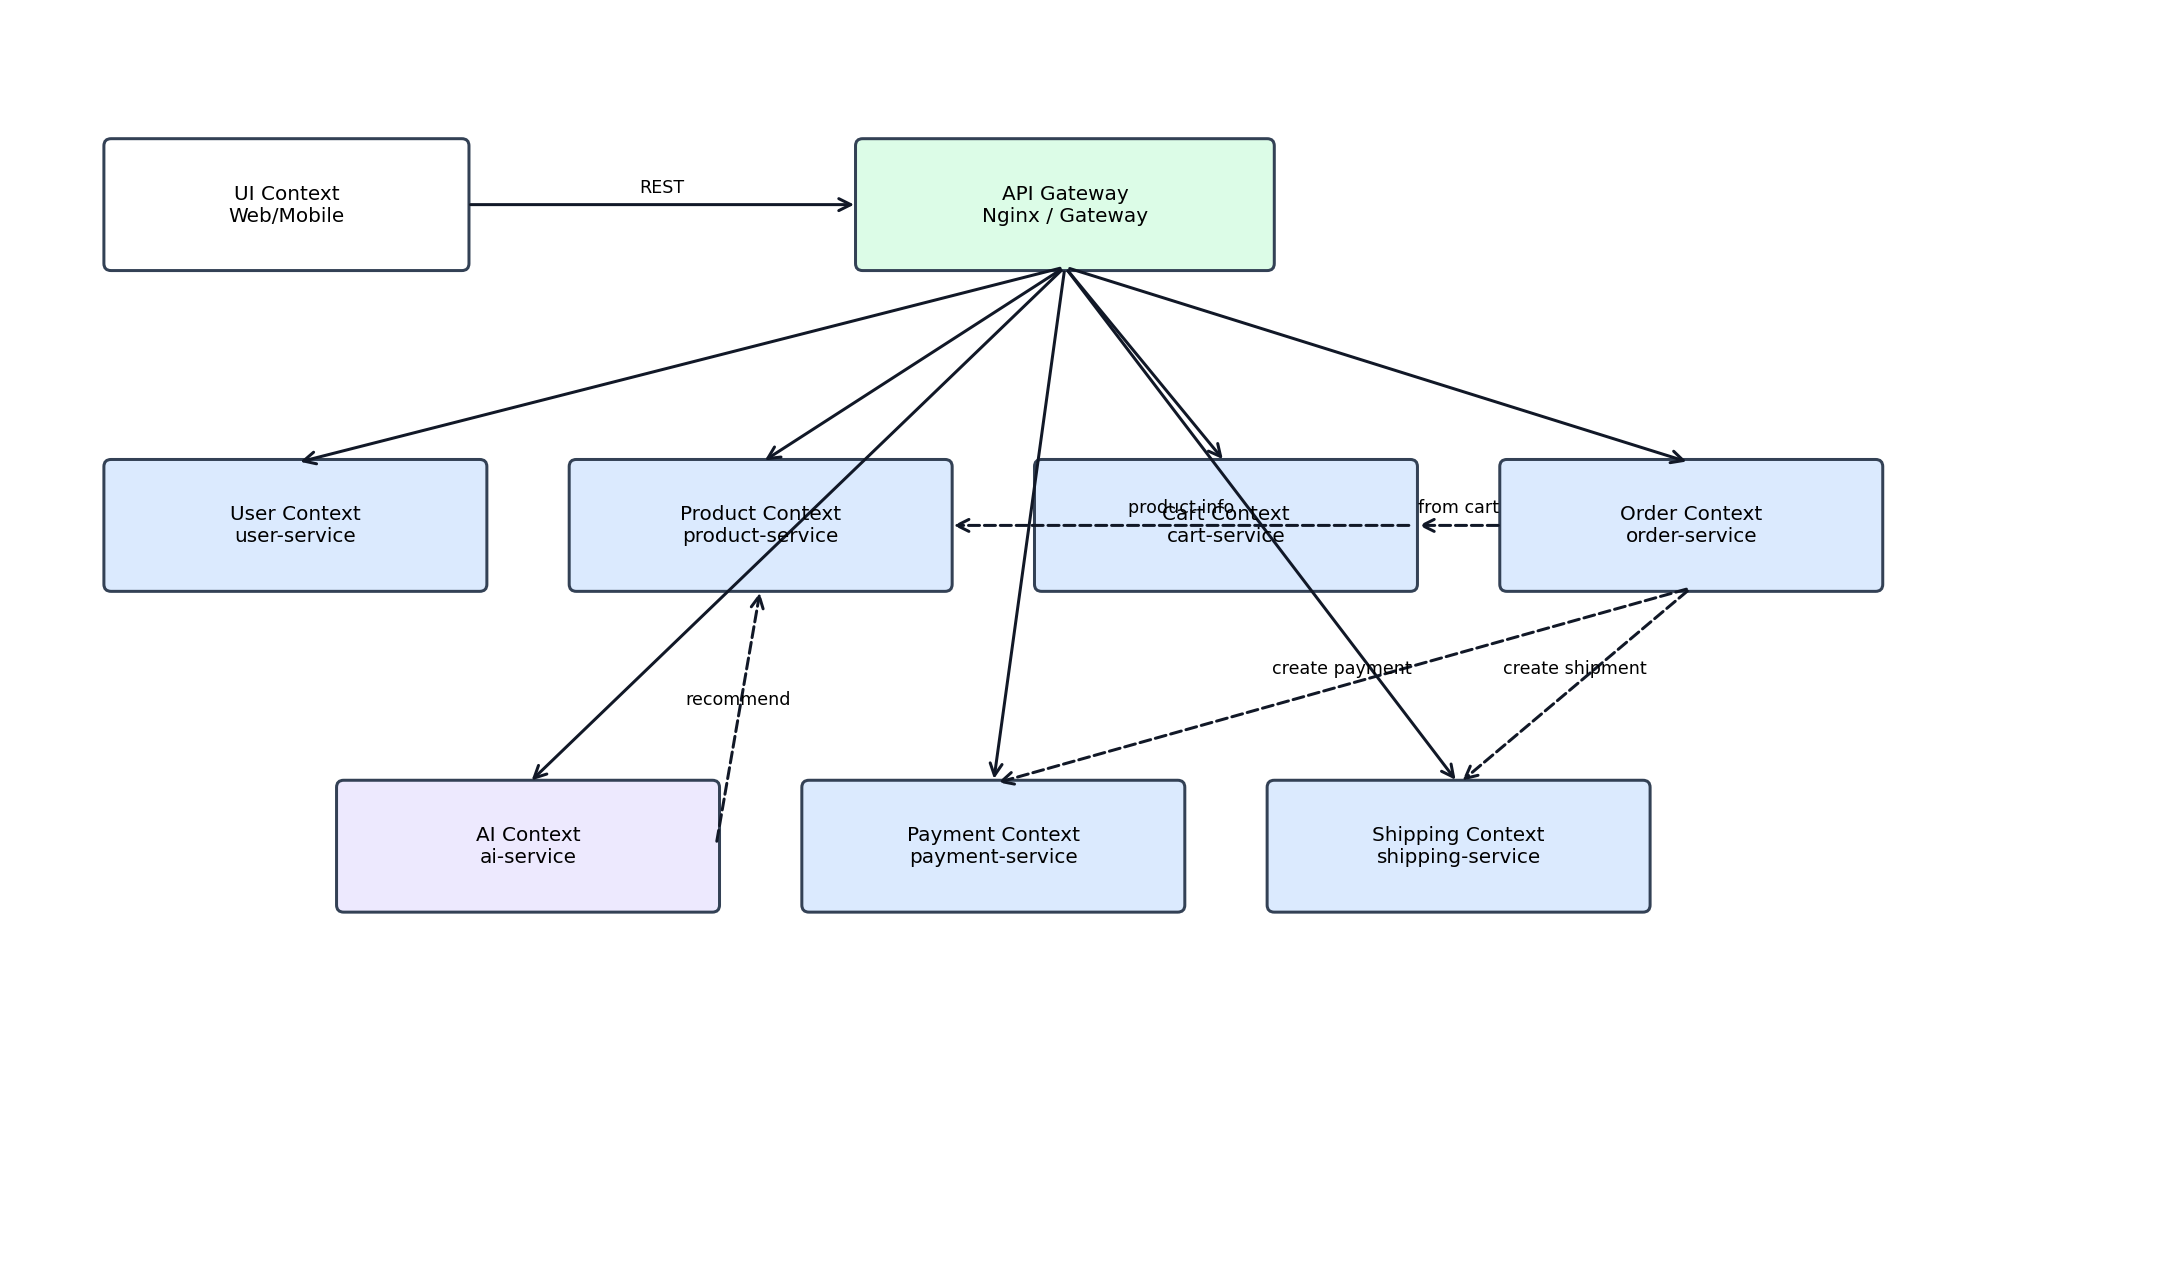
\includegraphics[width=0.95\linewidth]{generated_diagrams/ecom_context_map.png}
\caption{DDD context map for the target e-commerce system.}
\label{fig:ecom-context-map}
\end{figure}

\subsubsection{DDD in Microservices}

DDD is useful for microservices because one bounded context is often a good candidate for one microservice. This does not mean every class becomes a service. The goal is to group behavior and data that change together.

\subsection{Case Study: Healthcare (Practice Decomposition)}

\subsubsection{Problem Description}

Healthcare is used here only as a decomposition case study, not as the main project of the essay. The purpose is to practice DDD thinking in a domain that has multiple business capabilities, such as patient identity, appointment, medical record, billing, pharmacy, and notification.

\subsubsection{Step 1: Identify the Domain}

The domain is a healthcare service system. The core business goal is to help users receive healthcare services safely and traceably. The system may contain patient registration, appointment booking, medical record management, pharmacy support, billing, and notification.

\subsubsection{Step 2: Identify Bounded Contexts}

The healthcare domain can be decomposed into these bounded contexts:

\begin{itemize}
    \item Patient/User Context.
    \item Appointment Context.
    \item Medical Record Context.
    \item Pharmacy Context.
    \item Billing Context.
    \item Notification Context.
\end{itemize}

\subsubsection{Step 3: Decompose into Microservices}

\begin{figure}[H]
\centering
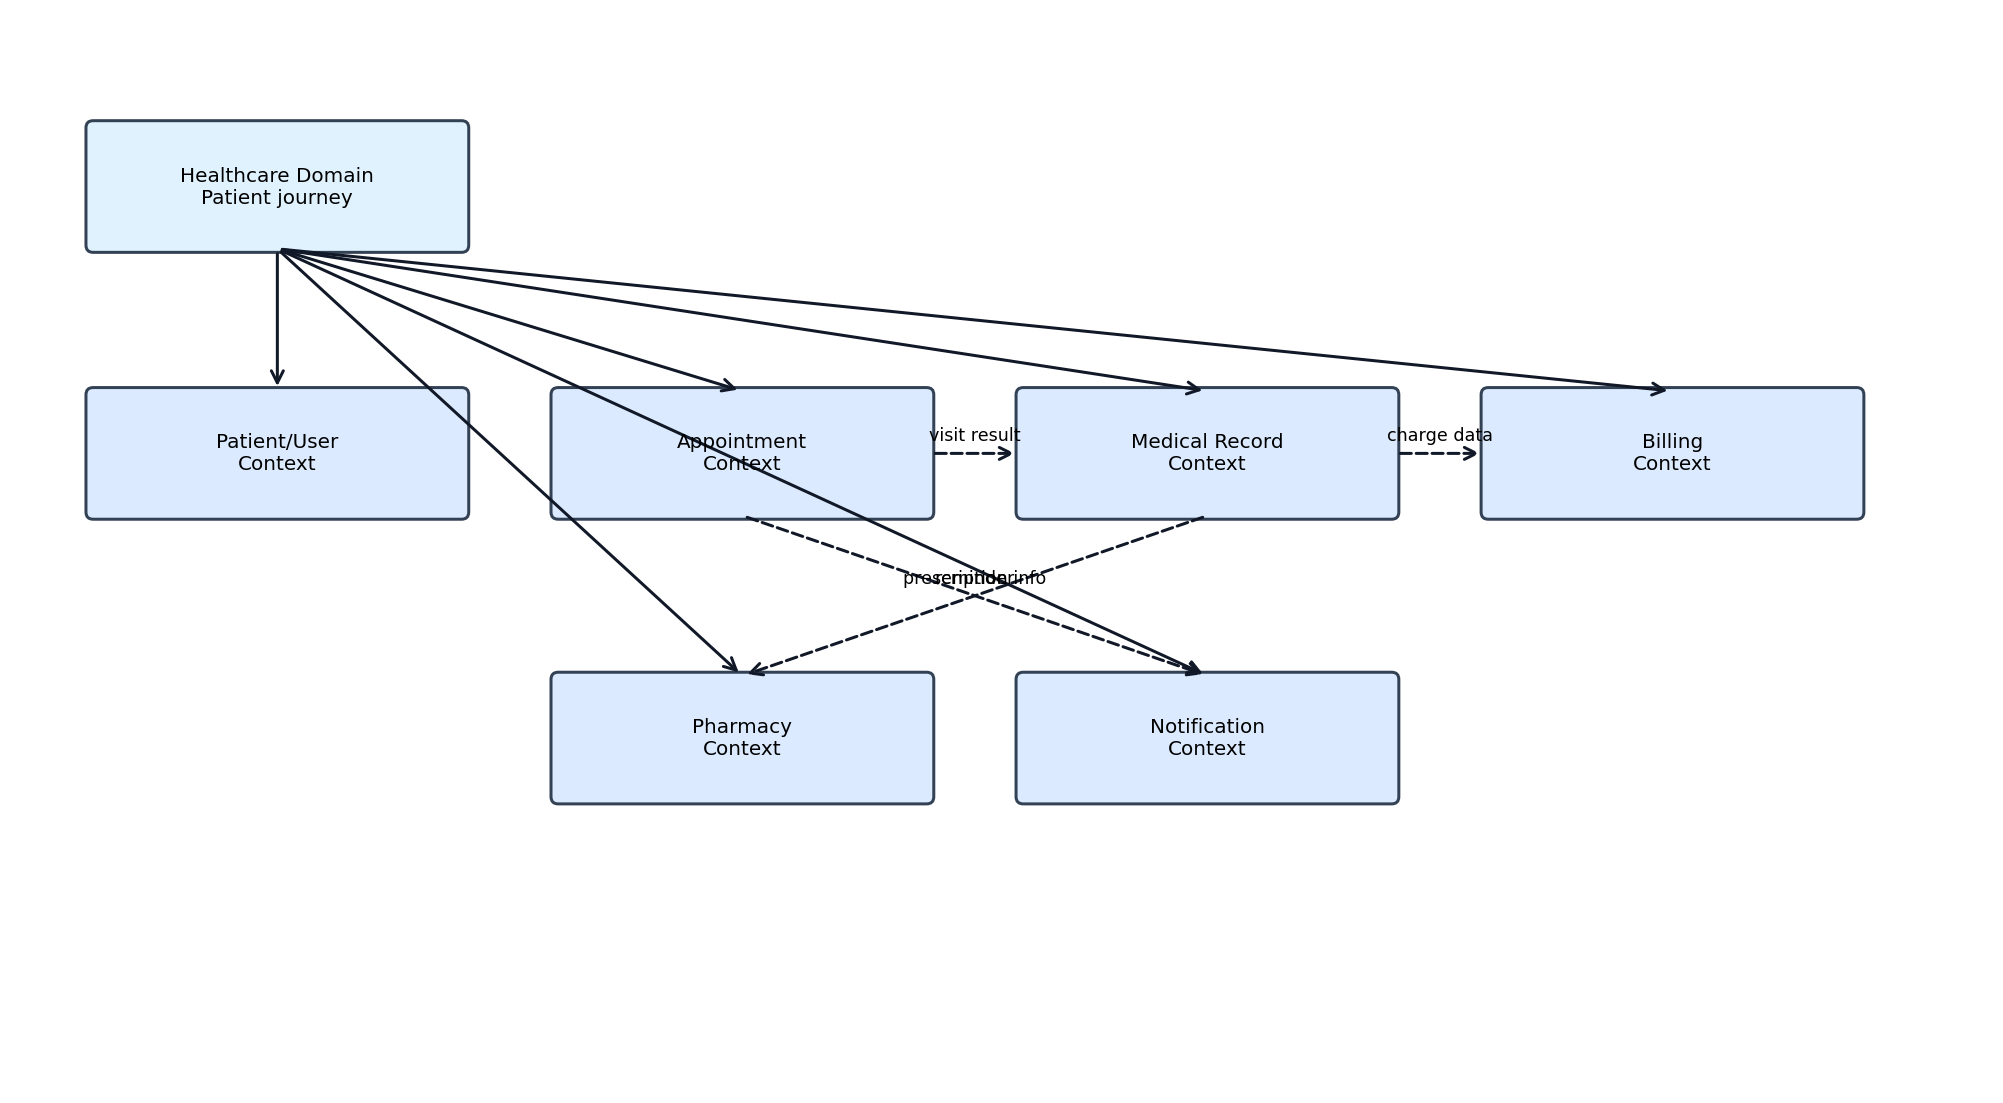
\includegraphics[width=0.92\linewidth]{generated_diagrams/healthcare_case_decomposition.png}
\caption{Healthcare case study decomposition for DDD practice.}
\label{fig:healthcare-case}
\end{figure}

Each context can become a service if it has enough independent business behavior. For example, appointment scheduling and billing should not share one database model because their business rules change for different reasons.

\subsubsection{Step 4: Identify Relationships}

The Appointment Context may call Notification to send reminders. The Medical Record Context may produce billing information. The Pharmacy Context may consume prescription-related information. These interactions should happen through APIs, not through direct database access.

\subsubsection{Example API}

\begin{lstlisting}[caption={Example healthcare API decomposition.}]
POST /api/patients/
POST /api/appointments/
GET  /api/medical-records/{patient_id}/
POST /api/pharmacy/dispense-requests/
POST /api/billing/invoices/
\end{lstlisting}

\subsection{Conclusion}

Monolithic architecture is suitable for simple early systems, but microservices are more appropriate when the system grows and the domain has clear boundaries. DDD provides a systematic way to identify those boundaries before creating services.

\section{Developing an E-Commerce Microservices System}

\subsection{Requirement Identification}

\subsubsection{Functional Requirements}

The main project is a general e-commerce system. It should support:

\begin{itemize}
    \item Product management across multiple product domains such as books, electronics, and fashion.
    \item User management for admin, staff, and customer roles.
    \item Cart management.
    \item Order creation and order history.
    \item Payment processing or simulated payment.
    \item Shipping and delivery tracking.
    \item Product search and recommendation.
    \item AI-assisted product consultation through recommendation list and chatbot.
\end{itemize}

\subsubsection{Non-functional Requirements}

\begin{itemize}
    \item \textbf{Scalability}: services can be scaled independently.
    \item \textbf{Security}: JWT authentication, role-based access control, and gateway validation.
    \item \textbf{Maintainability}: business logic is separated by bounded context.
    \item \textbf{Availability}: service failures should be isolated where possible.
    \item \textbf{Deployability}: Docker Compose should run the system locally.
\end{itemize}

\subsection{DDD-Based System Decomposition}

\subsubsection{Bounded Contexts}

\begin{longtable}{p{0.26\linewidth}p{0.28\linewidth}p{0.36\linewidth}}
\caption{E-commerce bounded contexts and services.}
\label{tab:ecom-bounded-contexts}\\
\toprule
\textbf{Bounded context} & \textbf{Service} & \textbf{Responsibility}\\
\midrule
\endfirsthead
\toprule
\textbf{Bounded context} & \textbf{Service} & \textbf{Responsibility}\\
\midrule
\endhead
User Context & \codepath{user-service} & Authentication, authorization, profiles, roles\\
Product Context & \codepath{product-service} & Categories, products, inventory, search\\
Cart Context & \codepath{cart-service} & Cart, cart items, quantity updates\\
Order Context & \codepath{order-service} & Order creation, order items, order lifecycle\\
Payment Context & \codepath{payment-service} & Payment records, payment status, confirmation\\
Shipping Context & \codepath{shipping-service} & Shipment creation and delivery status\\
AI Context & \codepath{ai-service} & Product recommendation and chatbot consultation\\
\bottomrule
\end{longtable}

\subsubsection{Principles}

\begin{itemize}
    \item Each context owns its own database.
    \item Services communicate through REST APIs.
    \item Frontend clients call through the API Gateway.
    \item No service should directly read or write another service's database.
\end{itemize}

\subsection{Product Service Design (Django)}

\subsubsection{Product Classification}

The product service supports multiple product domains:

\begin{itemize}
    \item Book: textbooks, novels, reference books.
    \item Electronics: mobile phones, laptops, home appliances.
    \item Fashion: shirts, pants, shoes, accessories.
\end{itemize}

\subsubsection{General Model}

\begin{lstlisting}[language=Python,caption={General product model.}]
class Category(models.Model):
    name = models.CharField(max_length=100)

class Product(models.Model):
    name = models.CharField(max_length=255)
    price = models.FloatField()
    stock = models.IntegerField()
    category = models.ForeignKey(Category, on_delete=models.CASCADE)
\end{lstlisting}

\subsubsection{Domain-Specific Details}

\begin{lstlisting}[language=Python,caption={Domain-specific product extensions.}]
class Book(models.Model):
    product = models.OneToOneField(Product, on_delete=models.CASCADE)
    author = models.CharField(max_length=255)
    publisher = models.CharField(max_length=255)
    isbn = models.CharField(max_length=20)

class Electronics(models.Model):
    product = models.OneToOneField(Product, on_delete=models.CASCADE)
    brand = models.CharField(max_length=100)
    warranty = models.IntegerField()

class Fashion(models.Model):
    product = models.OneToOneField(Product, on_delete=models.CASCADE)
    size = models.CharField(max_length=10)
    color = models.CharField(max_length=50)
\end{lstlisting}

\subsubsection{API}

\begin{lstlisting}[caption={Product service API.}]
GET  /products/
POST /products/
GET  /products/{id}/
PUT  /products/{id}/
DELETE /products/{id}/
\end{lstlisting}

\subsection{User Service Design (Django)}

\subsubsection{User Classification}

The user service supports three roles:

\begin{itemize}
    \item Admin: full system management.
    \item Staff: product, order, and shipping operations.
    \item Customer: product browsing, cart, checkout, and order history.
\end{itemize}

\subsubsection{Model}

\begin{lstlisting}[language=Python,caption={User role model.}]
from django.contrib.auth.models import AbstractUser

class User(AbstractUser):
    ROLE_CHOICES = (
        ("admin", "Admin"),
        ("staff", "Staff"),
        ("customer", "Customer"),
    )
    role = models.CharField(max_length=20, choices=ROLE_CHOICES)
\end{lstlisting}

\subsubsection{Role-Based Access Control}

Admin can manage the whole system. Staff can process orders, update products, and manage shipping. Customers can browse products, manage cart, place orders, and view their own order history.

\subsubsection{API}

\begin{lstlisting}[caption={User service API.}]
POST /auth/register/
POST /auth/login/
GET  /users/
GET  /users/me/
\end{lstlisting}

\subsection{Cart Service Design}

\subsubsection{Model}

\begin{lstlisting}[language=Python,caption={Cart service model.}]
class Cart(models.Model):
    user_id = models.IntegerField()

class CartItem(models.Model):
    cart = models.ForeignKey(Cart, on_delete=models.CASCADE)
    product_id = models.IntegerField()
    quantity = models.IntegerField()
\end{lstlisting}

\subsubsection{Logic}

The cart service handles adding products, updating quantity, removing items, and returning the current customer cart. It stores product identifiers but should not directly access the product database.

\subsubsection{API}

\begin{lstlisting}[caption={Cart service API.}]
POST   /cart/add/
GET    /cart/
PATCH  /cart/items/{id}/
DELETE /cart/remove/{id}/
\end{lstlisting}

\subsection{Order Service Design}

\subsubsection{Model}

\begin{lstlisting}[language=Python,caption={Order service model.}]
class Order(models.Model):
    user_id = models.IntegerField()
    total_price = models.FloatField()
    status = models.CharField(max_length=50)

class OrderItem(models.Model):
    order = models.ForeignKey(Order, on_delete=models.CASCADE)
    product_id = models.IntegerField()
    quantity = models.IntegerField()
\end{lstlisting}

\subsubsection{Workflow}

The order service creates an order from the cart, stores order items, calls the payment service, and then calls the shipping service. For a robust design, order items should store product snapshots so that historical orders do not change when product information changes.

\subsection{Payment Service Design}

\subsubsection{Model}

\begin{lstlisting}[language=Python,caption={Payment service model.}]
class Payment(models.Model):
    order_id = models.IntegerField()
    amount = models.FloatField()
    status = models.CharField(max_length=50)
\end{lstlisting}

\subsubsection{States}

Payment status can be \codepath{pending}, \codepath{success}, or \codepath{failed}. A more detailed implementation may use \codepath{pending}, \codepath{paid}, \codepath{failed}, and \codepath{cancelled}.

\subsubsection{API}

\begin{lstlisting}[caption={Payment service API.}]
POST /payment/pay/
GET  /payment/status/{id}/
\end{lstlisting}

\subsection{Shipping Service Design}

\subsubsection{Model}

\begin{lstlisting}[language=Python,caption={Shipping service model.}]
class Shipment(models.Model):
    order_id = models.IntegerField()
    address = models.TextField()
    status = models.CharField(max_length=50)
\end{lstlisting}

\subsubsection{States}

Shipping status can be \codepath{processing}, \codepath{shipping}, and \codepath{delivered}. A more complete design can include \codepath{pending}, \codepath{preparing}, \codepath{shipped}, \codepath{delivered}, and \codepath{cancelled}.

\subsubsection{API}

\begin{lstlisting}[caption={Shipping service API.}]
POST /shipping/create/
GET  /shipping/status/{id}/
PATCH /shipping/status/{id}/
\end{lstlisting}

\subsection{Overall System Flow}

\begin{enumerate}[label=\arabic*.]
    \item User logs in through user-service.
    \item User browses products through product-service.
    \item User adds products to cart through cart-service.
    \item User checks out and creates an order through order-service.
    \item Order-service sends payment request to payment-service.
    \item After payment succeeds, order-service creates shipment through shipping-service.
\end{enumerate}

\subsection{Practical Design Guide}

\subsubsection{Goal}

The practical design part should include class diagrams, database mapping, and database design per service. This is required because the essay is not only theoretical; it must show how microservices are mapped into concrete design artifacts.

\subsubsection{Class Diagram}

\begin{figure}[H]
\centering
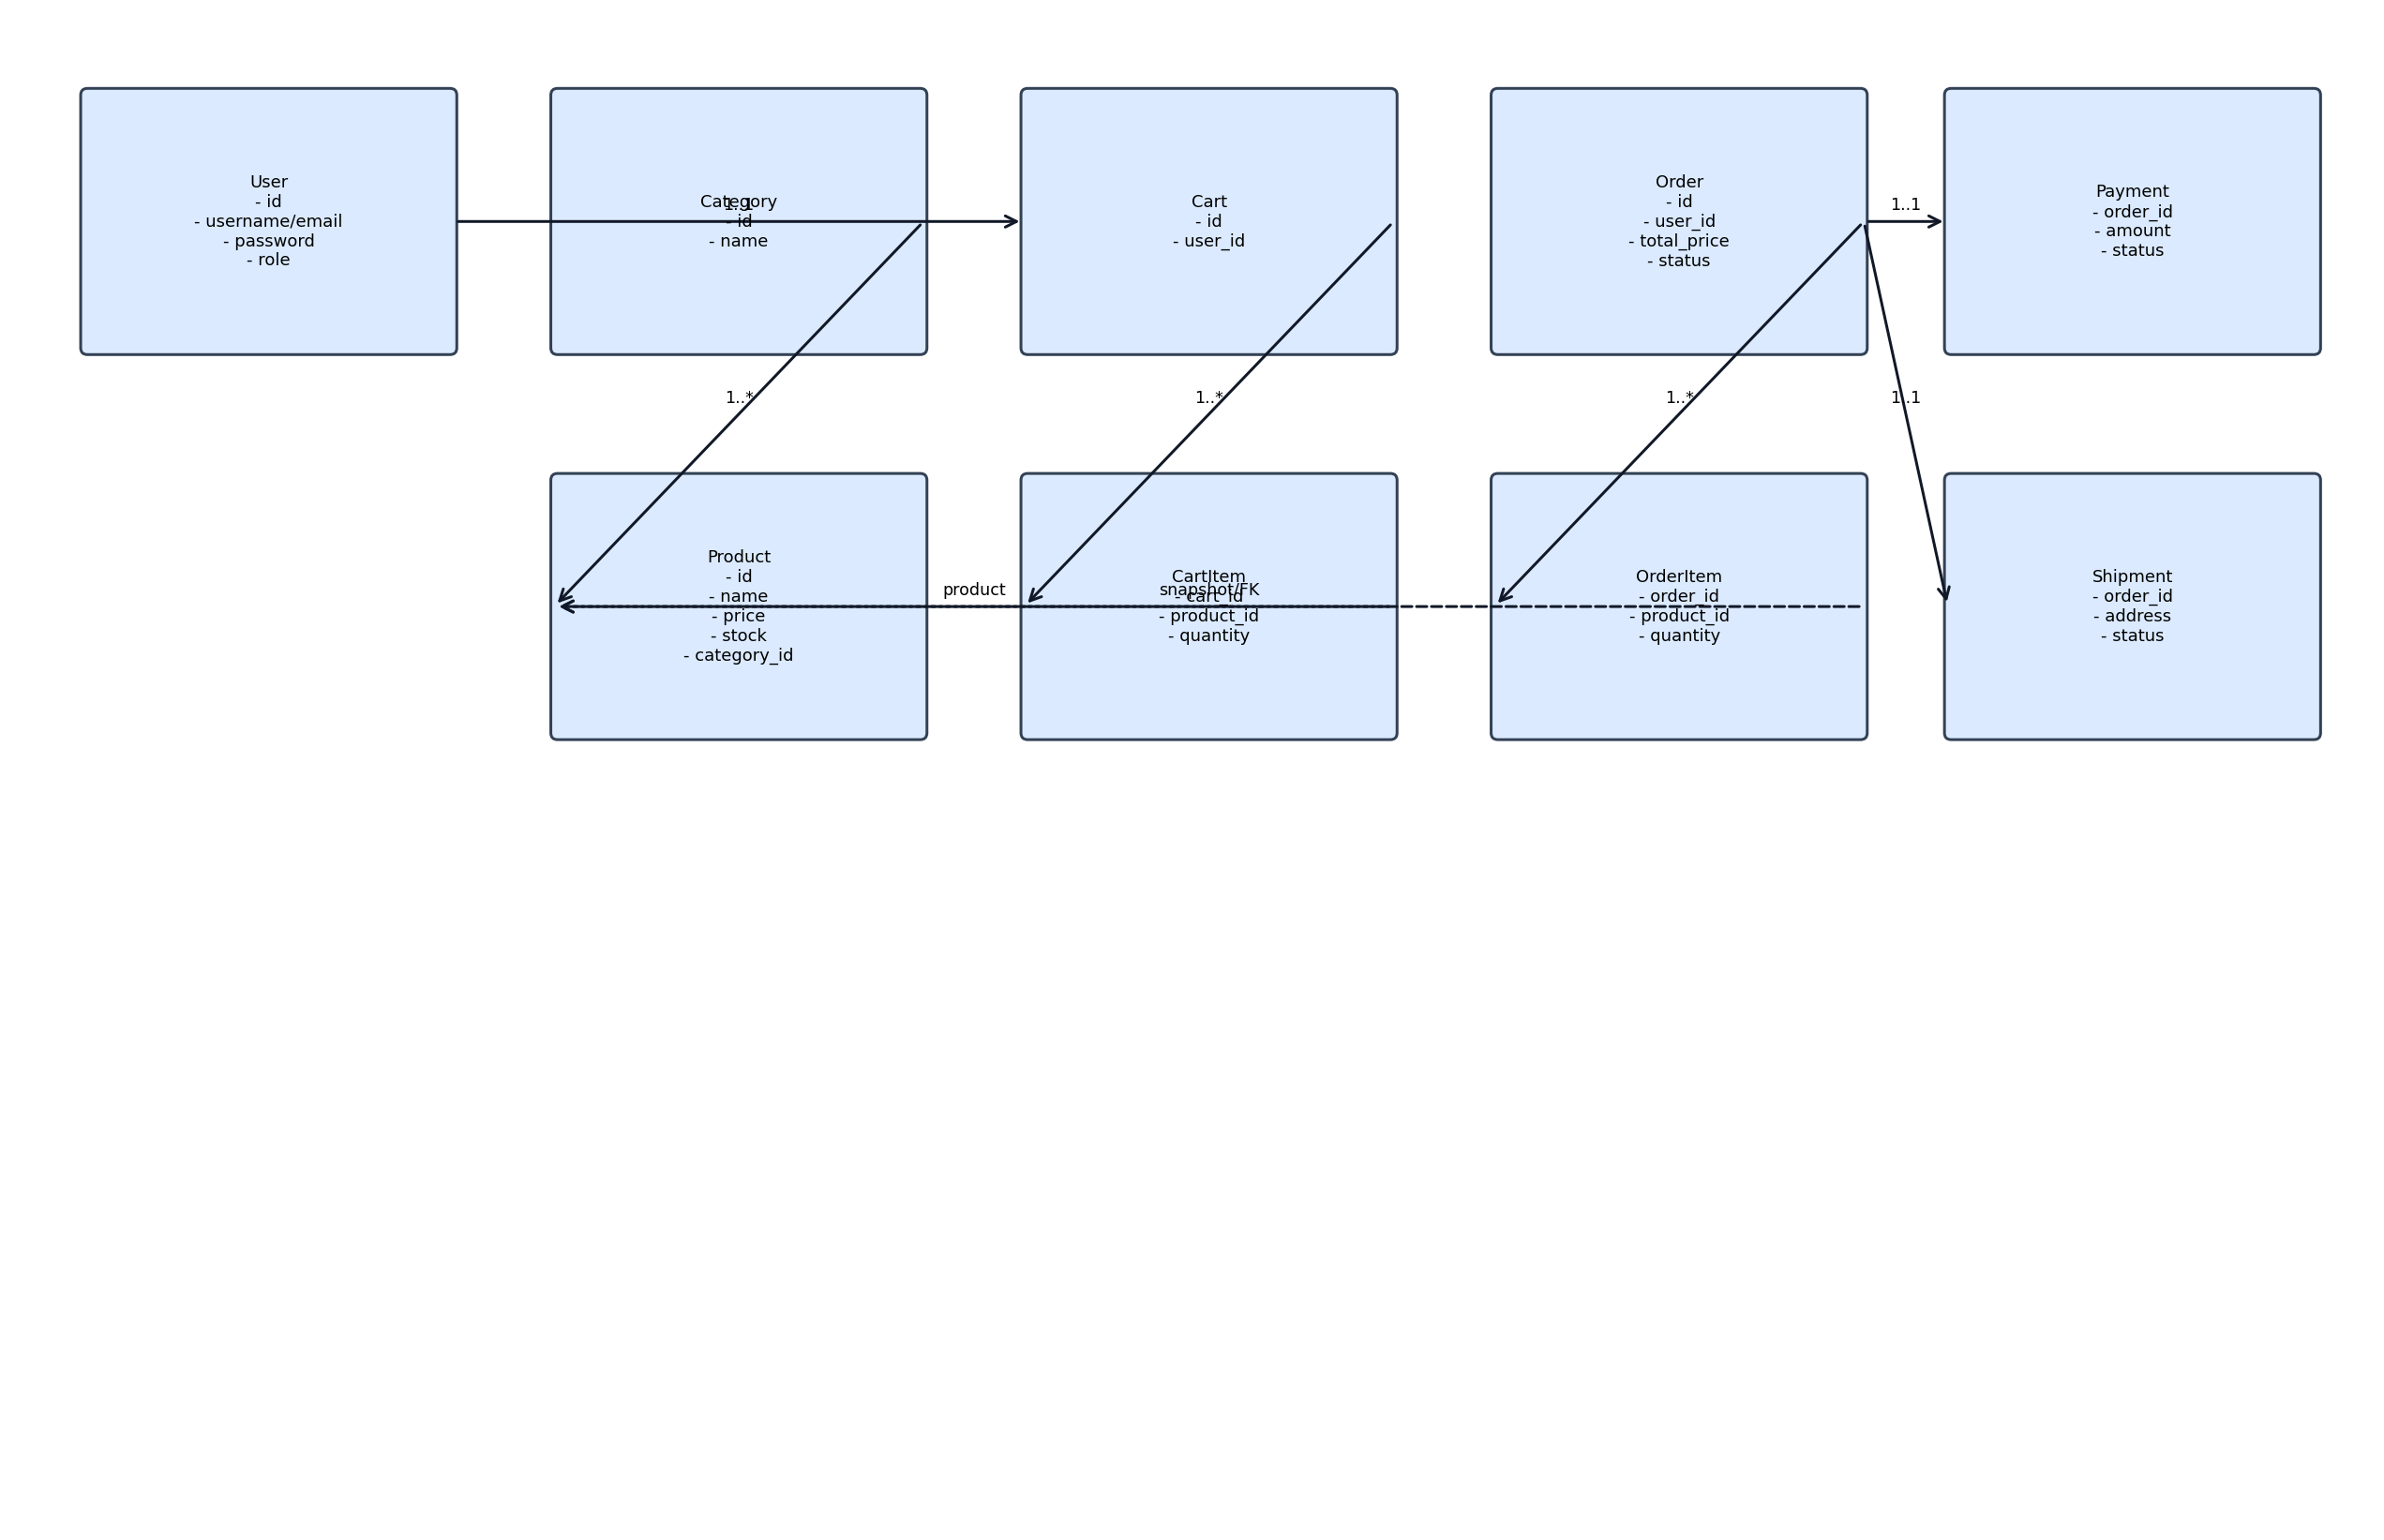
\includegraphics[width=0.98\linewidth]{generated_diagrams/ecom_class_diagram.png}
\caption{Class diagram for the target e-commerce microservices system.}
\label{fig:ecom-class-diagram}
\end{figure}

\subsubsection{Mapping Class Diagram to Database}

The general mapping rule is:

\begin{itemize}
    \item Class maps to table.
    \item Attribute maps to column.
    \item Relationship maps to foreign key or service-level identifier.
    \item Cross-service references should use IDs or snapshots, not direct database foreign keys.
\end{itemize}

\subsubsection{Database Design for Each Service}

\begin{figure}[H]
\centering
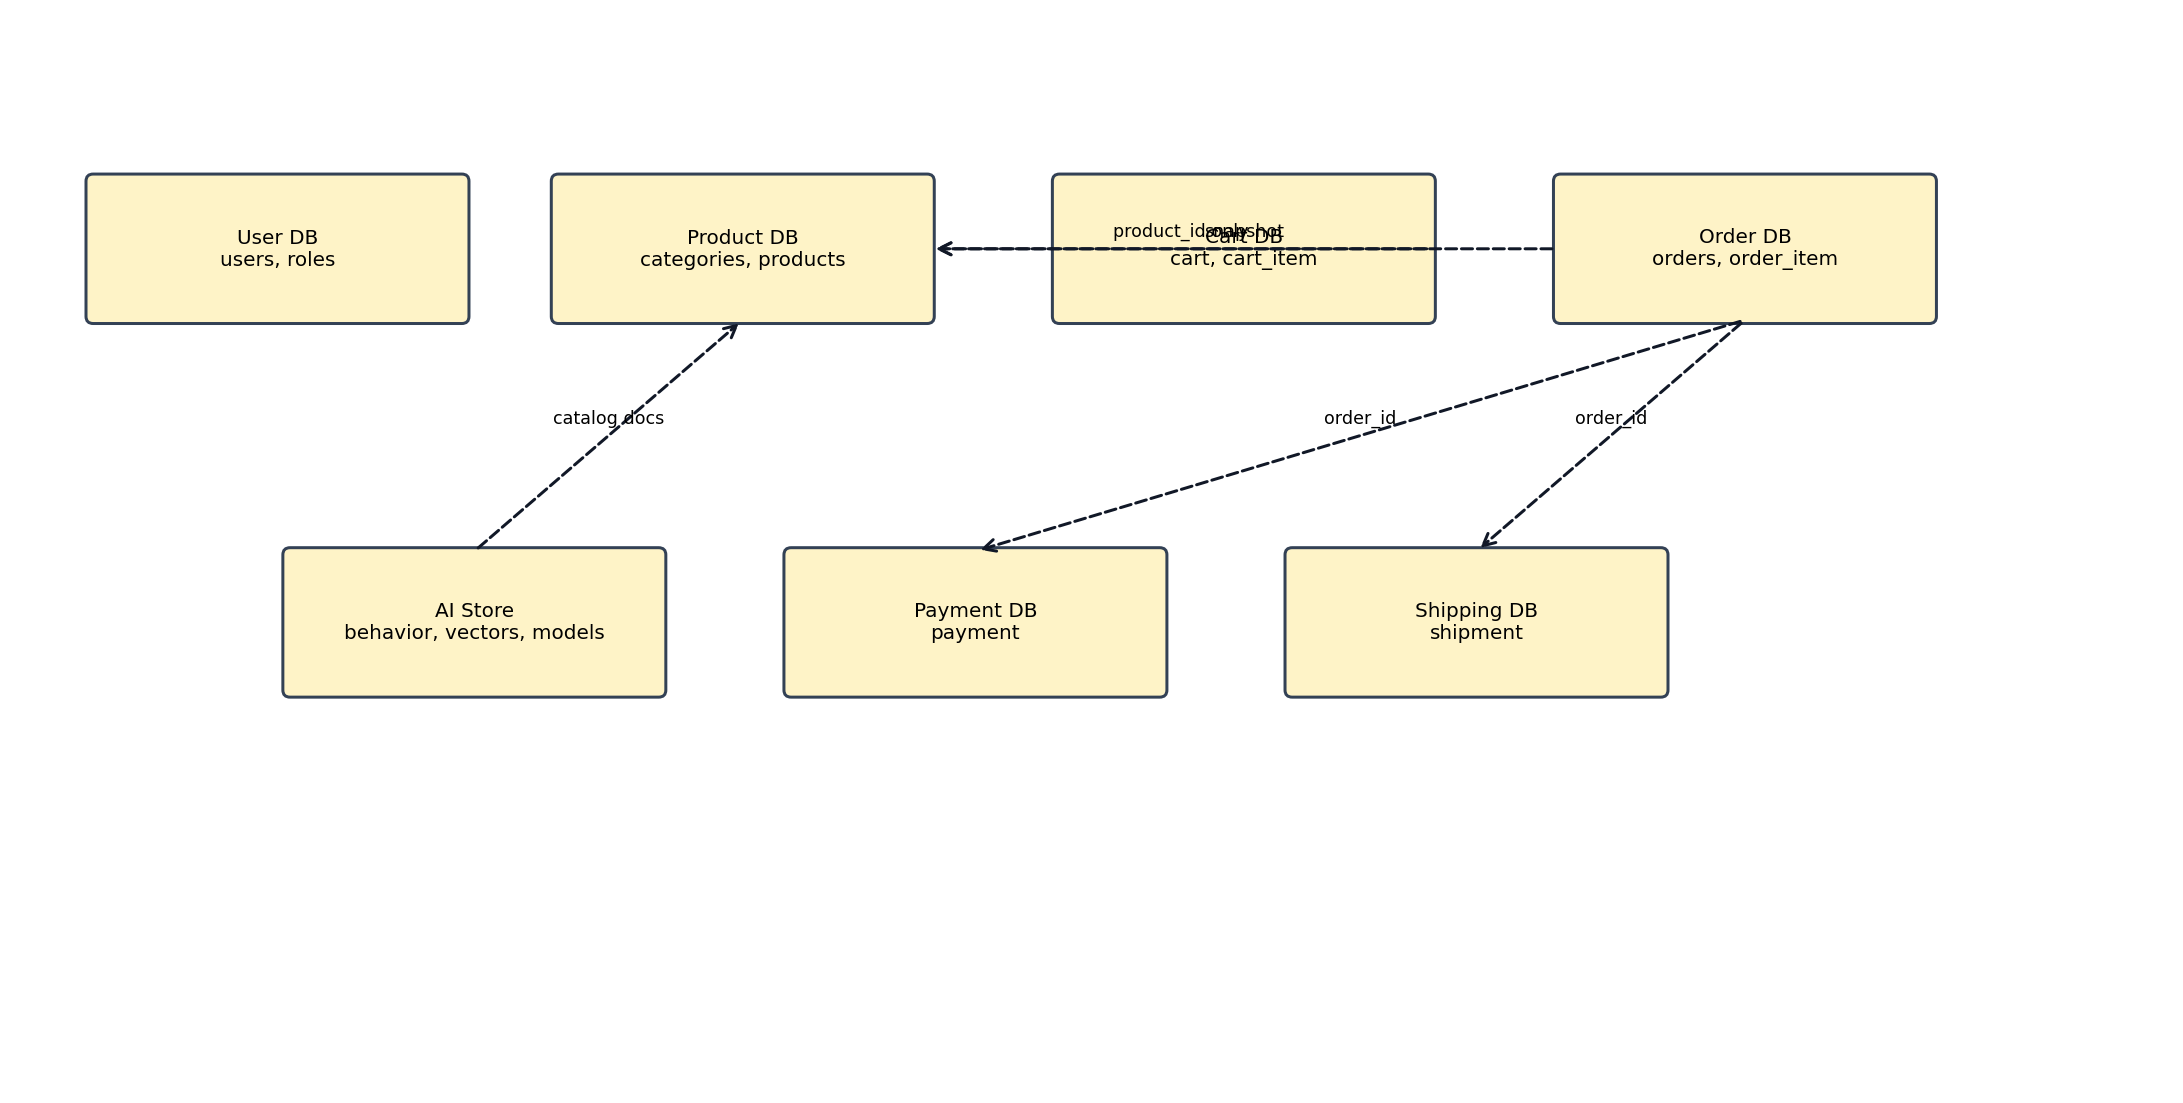
\includegraphics[width=0.92\linewidth]{generated_diagrams/ecom_database_mapping.png}
\caption{Database-per-service mapping for the target e-commerce system.}
\label{fig:ecom-db-mapping}
\end{figure}

\begin{longtable}{p{0.25\linewidth}p{0.25\linewidth}p{0.38\linewidth}}
\caption{Main database schema by service.}
\label{tab:ecom-db-schema}\\
\toprule
\textbf{Service} & \textbf{Suggested DB} & \textbf{Main tables}\\
\midrule
\endfirsthead
\toprule
\textbf{Service} & \textbf{Suggested DB} & \textbf{Main tables}\\
\midrule
\endhead
Product Service & PostgreSQL & category, product, book, electronics, fashion\\
User Service & MySQL & user, role, profile\\
Cart Service & MySQL or PostgreSQL & cart, cart\_item\\
Order Service & MySQL or PostgreSQL & orders, order\_item\\
Payment Service & PostgreSQL & payment\\
Shipping Service & PostgreSQL & shipment\\
AI Service & PostgreSQL + Vector DB/Files & behavior events, embeddings, model artifacts\\
\bottomrule
\end{longtable}

\subsubsection{MySQL vs PostgreSQL}

\begin{table}[H]
\centering
\caption{MySQL and PostgreSQL comparison.}
\label{tab:mysql-postgres}
\begin{tabular}{p{0.25\linewidth}p{0.30\linewidth}p{0.30\linewidth}}
\toprule
\textbf{Criteria} & \textbf{MySQL} & \textbf{PostgreSQL}\\
\midrule
Popularity & Very common for web applications & Very common for complex applications\\
JSON support & Good & Strong\\
Complex queries & Good & Stronger for advanced queries\\
Authentication data & Suitable & Suitable\\
Catalog/search data & Suitable & Often preferred\\
\bottomrule
\end{tabular}
\end{table}

\subsubsection{Exercise}

The final project evidence should export the class diagram from a diagram tool or include a clear generated diagram in the report. It should also show service-specific database schemas and explain why databases are not shared across services.

\subsubsection{Evaluation Checklist}

\begin{itemize}
    \item Class diagram is clear and uses correct relationships.
    \item Database mapping is clear.
    \item Each service owns its own database.
    \item MySQL and PostgreSQL choices are explained.
\end{itemize}

\subsection{Conclusion}

The e-commerce system can be decomposed into user, product, cart, order, payment, shipping, and AI services. DDD helps ensure that each service maps to a business context rather than a random technical module.

\section{AI Service for Product Consultation}

\subsection{Goal}

The AI service improves the e-commerce customer experience by recommending products and answering product consultation questions. It can use user behavior, product similarity, and natural-language query context.

Expected outputs are:

\begin{itemize}
    \item Recommended product list.
    \item Chatbot consultation response.
\end{itemize}

\subsection{AI Service Architecture}

The AI service is designed as an independent microservice. It receives user behavior and user queries, processes them through machine learning and retrieval components, and returns recommendations or chatbot responses.

\begin{figure}[H]
\centering
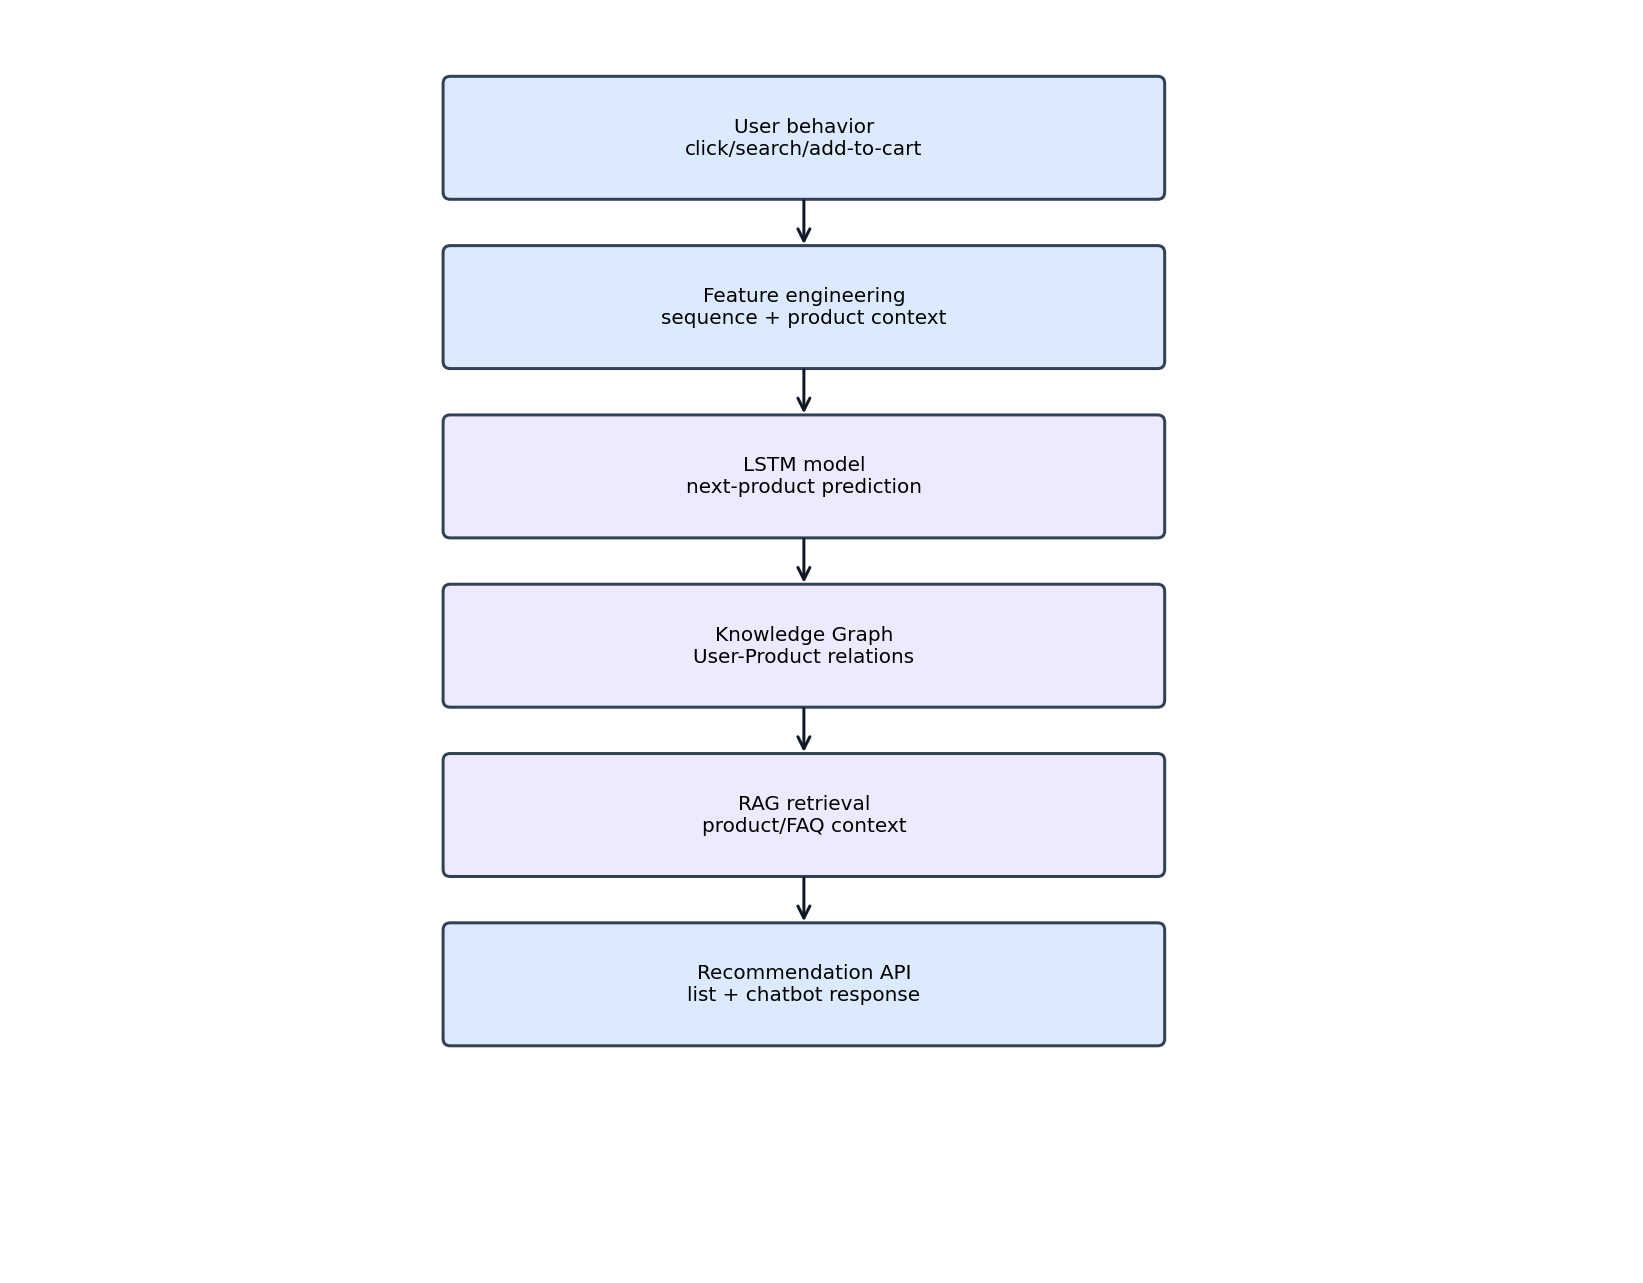
\includegraphics[width=0.75\linewidth]{generated_diagrams/ecom_ai_pipeline.png}
\caption{AI service pipeline for product consultation.}
\label{fig:ecom-ai-pipeline}
\end{figure}

\subsection{Data Collection}

\subsubsection{User Behavior Data}

The service can collect:

\begin{itemize}
    \item user\_id
    \item product\_id
    \item action: view, click, search, add\_to\_cart, buy
    \item timestamp
    \item query text or product category
\end{itemize}

\subsubsection{Example Dataset}

\begin{lstlisting}[caption={Example behavior dataset.}]
user_id,product_id,action,time
1,101,view,t1
1,102,add_to_cart,t2
2,205,buy,t3
\end{lstlisting}

\subsection{LSTM Model (Sequence Modeling)}

\subsubsection{Idea}

An LSTM model can predict the next product or category based on a sequence of user actions. For example, if a user views a phone, then views phone cases, then adds a charger to cart, the model may recommend related accessories.

\subsubsection{Detailed Model}

\begin{lstlisting}[language=Python,caption={Simplified LSTM recommendation model.}]
import torch
import torch.nn as nn

class LSTMModel(nn.Module):
    def __init__(self, input_dim=10, hidden_dim=64, output_dim=100):
        super().__init__()
        self.lstm = nn.LSTM(input_dim, hidden_dim, batch_first=True)
        self.fc = nn.Linear(hidden_dim, output_dim)

    def forward(self, x):
        out, _ = self.lstm(x)
        out = out[:, -1, :]
        return self.fc(out)
\end{lstlisting}

\subsubsection{Training}

\begin{lstlisting}[language=Python,caption={Simplified LSTM training loop.}]
criterion = nn.CrossEntropyLoss()
optimizer = torch.optim.Adam(model.parameters())

for epoch in range(epochs):
    output = model(x)
    loss = criterion(output, y)
    loss.backward()
    optimizer.step()
    optimizer.zero_grad()
\end{lstlisting}

\subsection{Knowledge Graph with Neo4j}

\subsubsection{Graph Model}

A knowledge graph can represent relationships between users, products, categories, and behavior.

\begin{itemize}
    \item Node types: User, Product, Category.
    \item Edge types: BUY, VIEW, ADD\_TO\_CART, SIMILAR, BELONGS\_TO.
\end{itemize}

\subsubsection{Cypher Example}

\begin{lstlisting}[caption={Neo4j Cypher example.}]
CREATE (u:User {id: 1})
CREATE (p:Product {id: 101})
CREATE (u)-[:BUY]->(p)
\end{lstlisting}

\subsubsection{Recommendation Query}

\begin{lstlisting}[caption={Graph recommendation query.}]
MATCH (u:User {id: 1})-[:BUY]->(p)-[:SIMILAR]->(rec)
RETURN rec
\end{lstlisting}

\subsection{RAG (Retrieval-Augmented Generation)}

\subsubsection{Pipeline}

RAG combines retrieval and generation. The retrieval step searches product documents, FAQ content, and product descriptions. The generation step uses the retrieved context to answer the user's question.

\subsubsection{Vector Database}

The vector database can be FAISS or ChromaDB. Product descriptions are converted into embeddings and searched by semantic similarity.

\subsubsection{Example}

\begin{lstlisting}[caption={RAG search example.}]
query = "cheap gaming laptop"
results = vector_db.search(query)
response = llm.generate(query, context=results)
\end{lstlisting}

\subsection{Hybrid Model}

A hybrid recommender can combine:

\begin{itemize}
    \item LSTM sequence score.
    \item Knowledge graph score.
    \item RAG semantic relevance score.
\end{itemize}

\begin{lstlisting}[caption={Hybrid recommendation score.}]
final_score = w1 * lstm_score + w2 * graph_score + w3 * rag_score
\end{lstlisting}

\subsection{Two AI Service Forms}

\subsubsection{Recommendation List}

Use cases:

\begin{itemize}
    \item Product search page.
    \item Product detail page.
    \item Cart page.
    \item Home dashboard.
\end{itemize}

\begin{lstlisting}[caption={Recommendation API.}]
GET /recommend?user_id=1

Response:
[101, 102, 205]
\end{lstlisting}

\subsubsection{Consultation Chatbot}

The chatbot receives a natural-language question, detects intent, retrieves product candidates, and generates a response.

\begin{lstlisting}[caption={Chatbot API.}]
POST /chatbot

Input:
"I need a cheap laptop for study"

Output:
"You may consider these budget laptop products..."
\end{lstlisting}

\subsection{AI Service Deployment}

\subsubsection{Tech Stack}

\begin{itemize}
    \item TensorFlow or PyTorch for LSTM.
    \item Neo4j for graph recommendation.
    \item FAISS or ChromaDB for vector retrieval.
    \item FastAPI or Django REST Framework for the AI service API.
\end{itemize}

\subsubsection{Architecture}

The AI service is independent and communicates with product and user behavior services through APIs. It should not directly modify product, cart, order, payment, or shipping databases.

\subsection{Exercise}

The AI exercise includes building a simple LSTM model, creating a product graph in Neo4j, implementing a recommendation API, and building a basic chatbot API.

\subsection{Evaluation Checklist}

\begin{itemize}
    \item AI pipeline is clear.
    \item At least one model is implemented.
    \item Graph and RAG design are explained.
    \item AI API is available.
    \item Recommendation output can be tested.
\end{itemize}

\subsection{Conclusion}

AI improves e-commerce personalization by using behavior, product relationships, and language context. In a microservice system, AI should remain a separate service so that model dependencies do not pollute core commerce services.

\section{Building the Complete System}

\subsection{Overall Architecture}

\subsubsection{System Model}

The complete system is built using microservices. Each service is a Django project or Python service and owns its data.

\begin{itemize}
    \item API Gateway (Nginx or dedicated gateway service).
    \item user-service.
    \item product-service.
    \item cart-service.
    \item order-service.
    \item payment-service.
    \item shipping-service.
    \item ai-service.
\end{itemize}

\subsubsection{Principles}

\begin{itemize}
    \item Each service owns a separate database.
    \item Services communicate through REST APIs.
    \item Services do not directly access each other's databases.
    \item The gateway is the single entry point for external clients.
\end{itemize}

\subsection{System Architecture}

\subsubsection{Overview}

The proposed e-commerce system is a distributed microservice-based platform. It supports product browsing, cart, checkout, payment, shipping, and AI-assisted product consultation.

\begin{figure}[H]
\centering
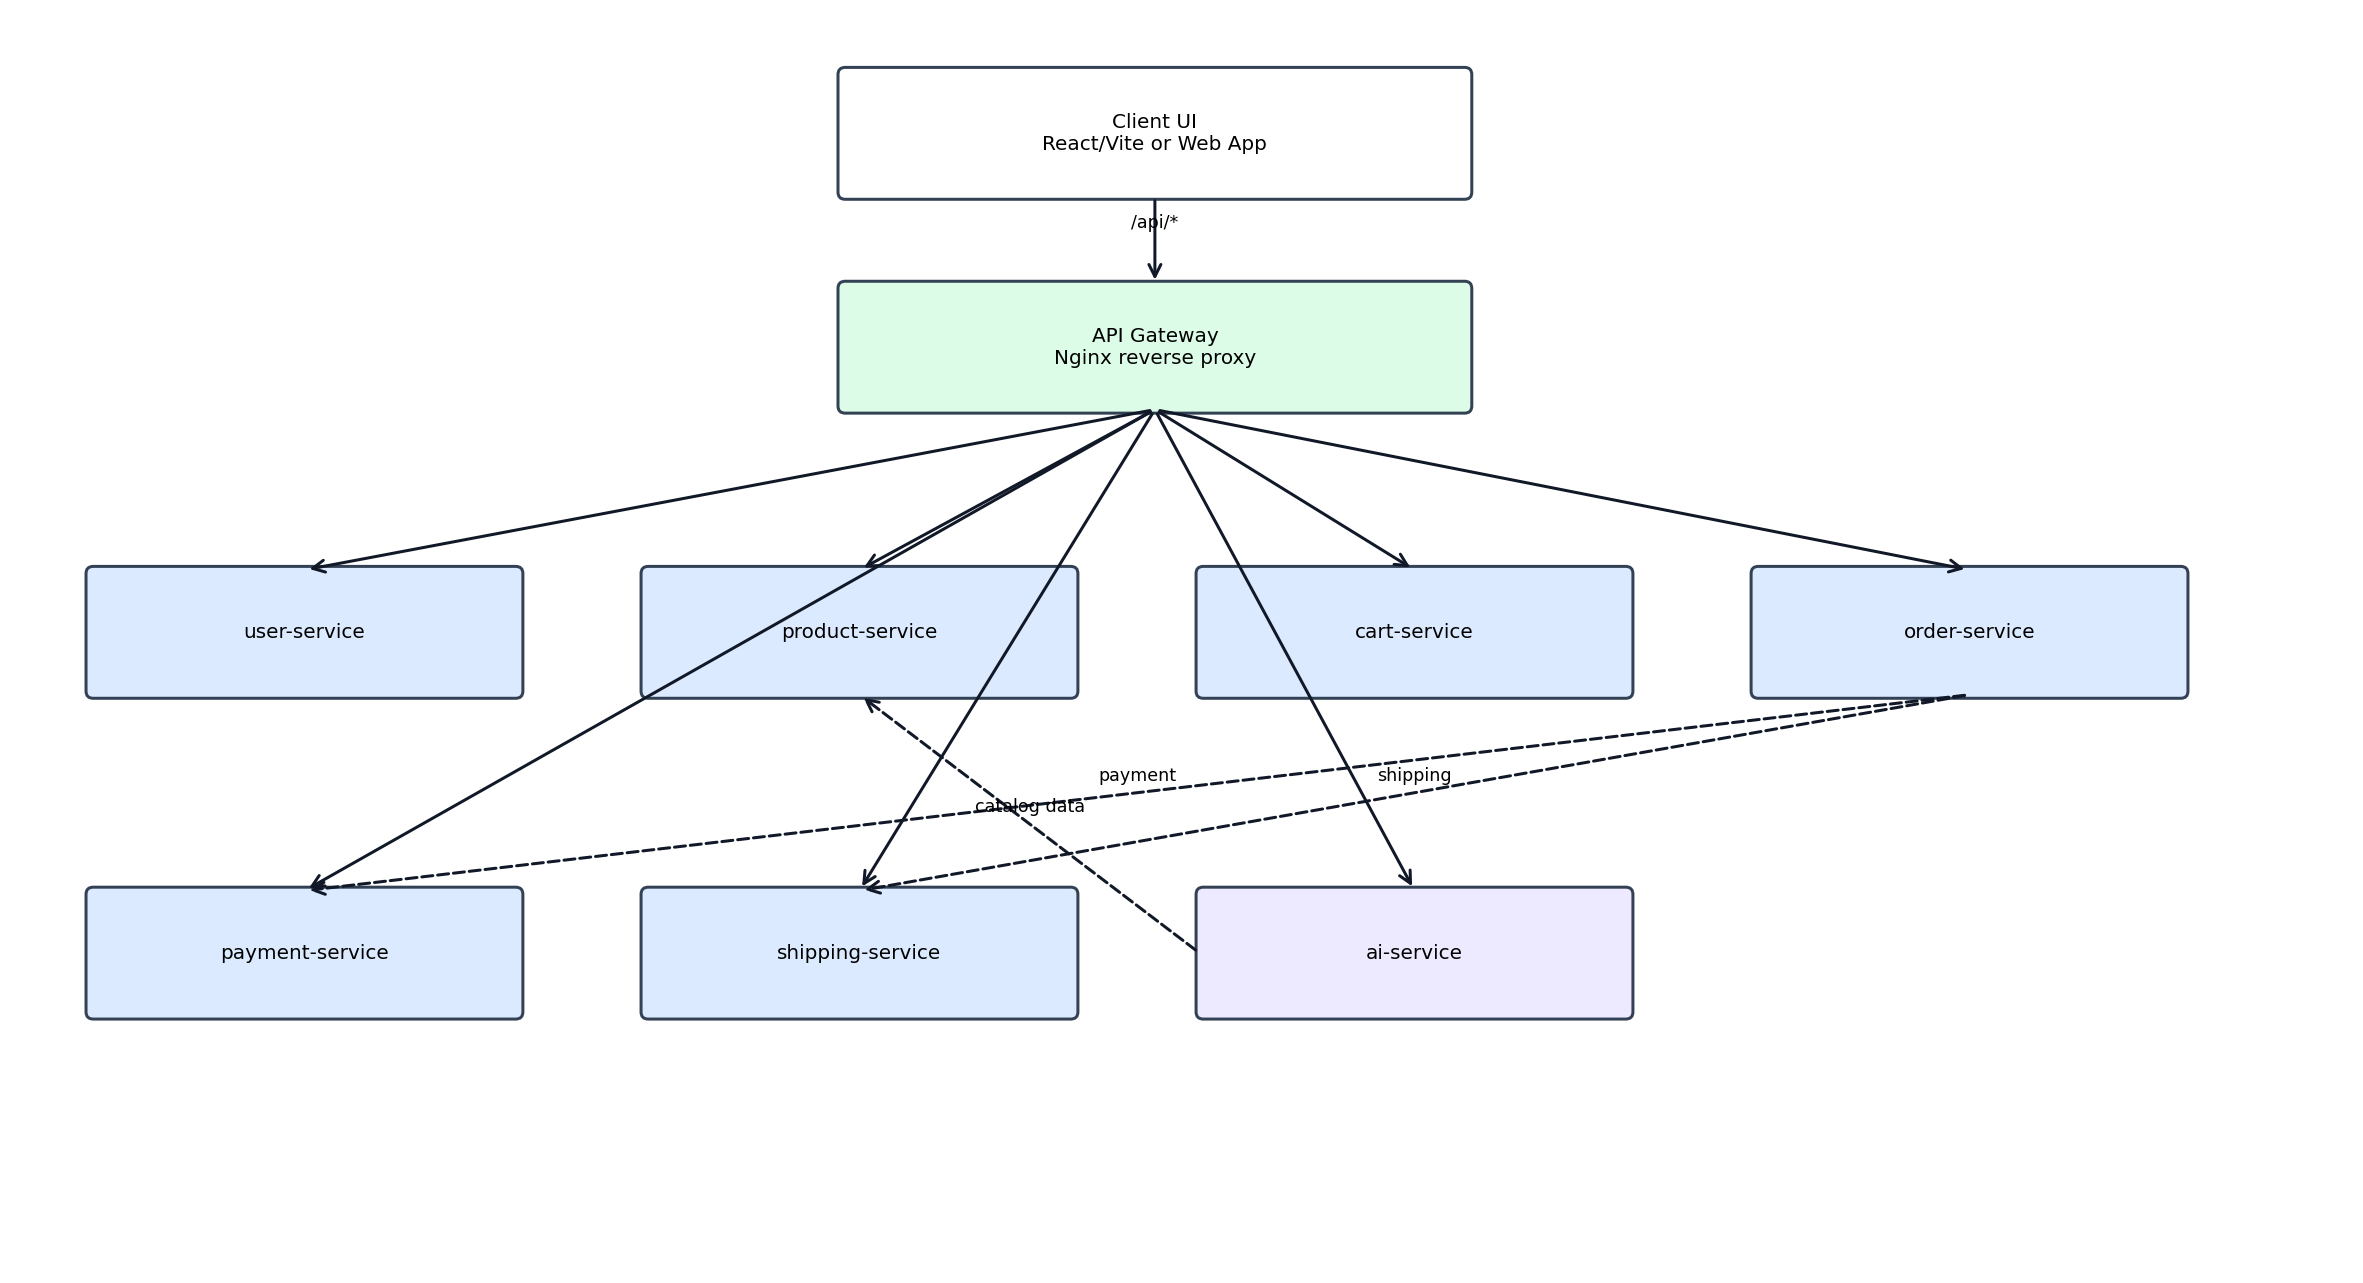
\includegraphics[width=0.98\linewidth]{generated_diagrams/ecom_system_architecture.png}
\caption{Microservice architecture of the target e-commerce system.}
\label{fig:ecom-system-architecture}
\end{figure}

\subsubsection{Microservice Architecture}

Each business domain is implemented as an independent service. The services are independently deployable and maintain their own databases. This follows the database-per-service pattern.

\subsubsection{API Gateway}

The API Gateway is the single entry point. It routes client requests to the correct service, forwards authentication headers, performs basic validation, and can centralize logging and monitoring.

\subsubsection{Service Communication}

For the MVP, synchronous REST APIs are acceptable. Later versions can add asynchronous communication with Redis, RabbitMQ, Kafka, or another message broker.

\subsubsection{Containerization and Deployment}

All services are containerized with Docker. Docker Compose is used for local development and demonstration. Kubernetes can be added later for production-style orchestration.

\subsubsection{System Structure}

\begin{lstlisting}[caption={Suggested project structure.}]
ecom-final/
|-- gateway/
|   |-- nginx.conf
|-- user-service/
|-- product-service/
|-- cart-service/
|-- order-service/
|-- payment-service/
|-- shipping-service/
|-- ai-service/
|-- infrastructure/
|   |-- docker-compose.yml
\end{lstlisting}

\subsubsection{Design Principles}

The architecture follows loose coupling, high cohesion, independent scalability, fault isolation, explicit API contracts, and database ownership.

\subsubsection{Security Considerations}

Security is enforced through JWT authentication, role-based access control, gateway validation, and service-level authorization. Staff and customer capabilities must be separated both in the UI and backend APIs.

\subsubsection{Discussion}

Compared with a monolithic architecture, the microservice design improves flexibility and scalability but introduces distributed-system complexity. Docker, API Gateway routing, clear service contracts, and observability reduce this complexity.

\subsection{API Gateway (Nginx)}

\subsubsection{Role}

The gateway is responsible for:

\begin{itemize}
    \item Acting as the entry point for the whole system.
    \item Routing requests to the correct service.
    \item Forwarding authentication headers.
    \item Logging API usage.
    \item Hiding internal service URLs from clients.
\end{itemize}

\subsubsection{Sample Configuration}

\begin{lstlisting}[caption={Sample Nginx gateway routing.}]
location /users/ {
    proxy_pass http://user-service:8000;
}

location /products/ {
    proxy_pass http://product-service:8001;
}

location /cart/ {
    proxy_pass http://cart-service:8002;
}
\end{lstlisting}

\subsection{Authentication (JWT)}

\subsubsection{Installation}

\begin{lstlisting}[caption={JWT dependency.}]
pip install djangorestframework-simplejwt
\end{lstlisting}

\subsubsection{Configuration}

\begin{lstlisting}[language=Python,caption={JWT view configuration.}]
from rest_framework_simplejwt.views import TokenObtainPairView
\end{lstlisting}

\subsubsection{Flow}

\begin{enumerate}[label=\arabic*.]
    \item User logs in and receives an access token.
    \item Client sends the token in the Authorization header.
    \item Gateway forwards the header.
    \item Service validates the token and role.
\end{enumerate}

\subsection{Communication Between Services}

\subsubsection{REST API Call}

\begin{lstlisting}[language=Python,caption={REST call between services.}]
import requests

response = requests.get(
    "http://product-service:8001/products/",
    timeout=5
)
\end{lstlisting}

\subsubsection{Best Practices}

\begin{itemize}
    \item Set request timeouts.
    \item Use retries carefully.
    \item Return clear errors.
    \item Use idempotency keys for payment and order operations.
    \item Add circuit breakers in advanced versions.
\end{itemize}

\subsection{Dockerizing the System}

\subsubsection{Dockerfile for Django}

\begin{lstlisting}[caption={Django Dockerfile.}]
FROM python:3.10
WORKDIR /app
COPY . .
RUN pip install -r requirements.txt
CMD ["python", "manage.py", "runserver", "0.0.0.0:8000"]
\end{lstlisting}

\subsubsection{docker-compose.yml}

\begin{lstlisting}[caption={Docker Compose sample.}]
version: "3"
services:
  user-service:
    build: ./user-service
    ports:
      - "8000:8000"

  product-service:
    build: ./product-service
    ports:
      - "8001:8001"
\end{lstlisting}

\subsection{End-to-End System Flow}

\subsubsection{Use Case: Shopping}

\begin{enumerate}[label=\arabic*.]
    \item User logs in through user-service.
    \item User views products through product-service.
    \item User adds product to cart through cart-service.
    \item User creates order through order-service.
    \item Order-service calls payment-service.
    \item Order-service calls shipping-service.
    \item AI-service can recommend related products during browsing or checkout.
\end{enumerate}

\subsubsection{Sequence Logic}

\begin{figure}[H]
\centering
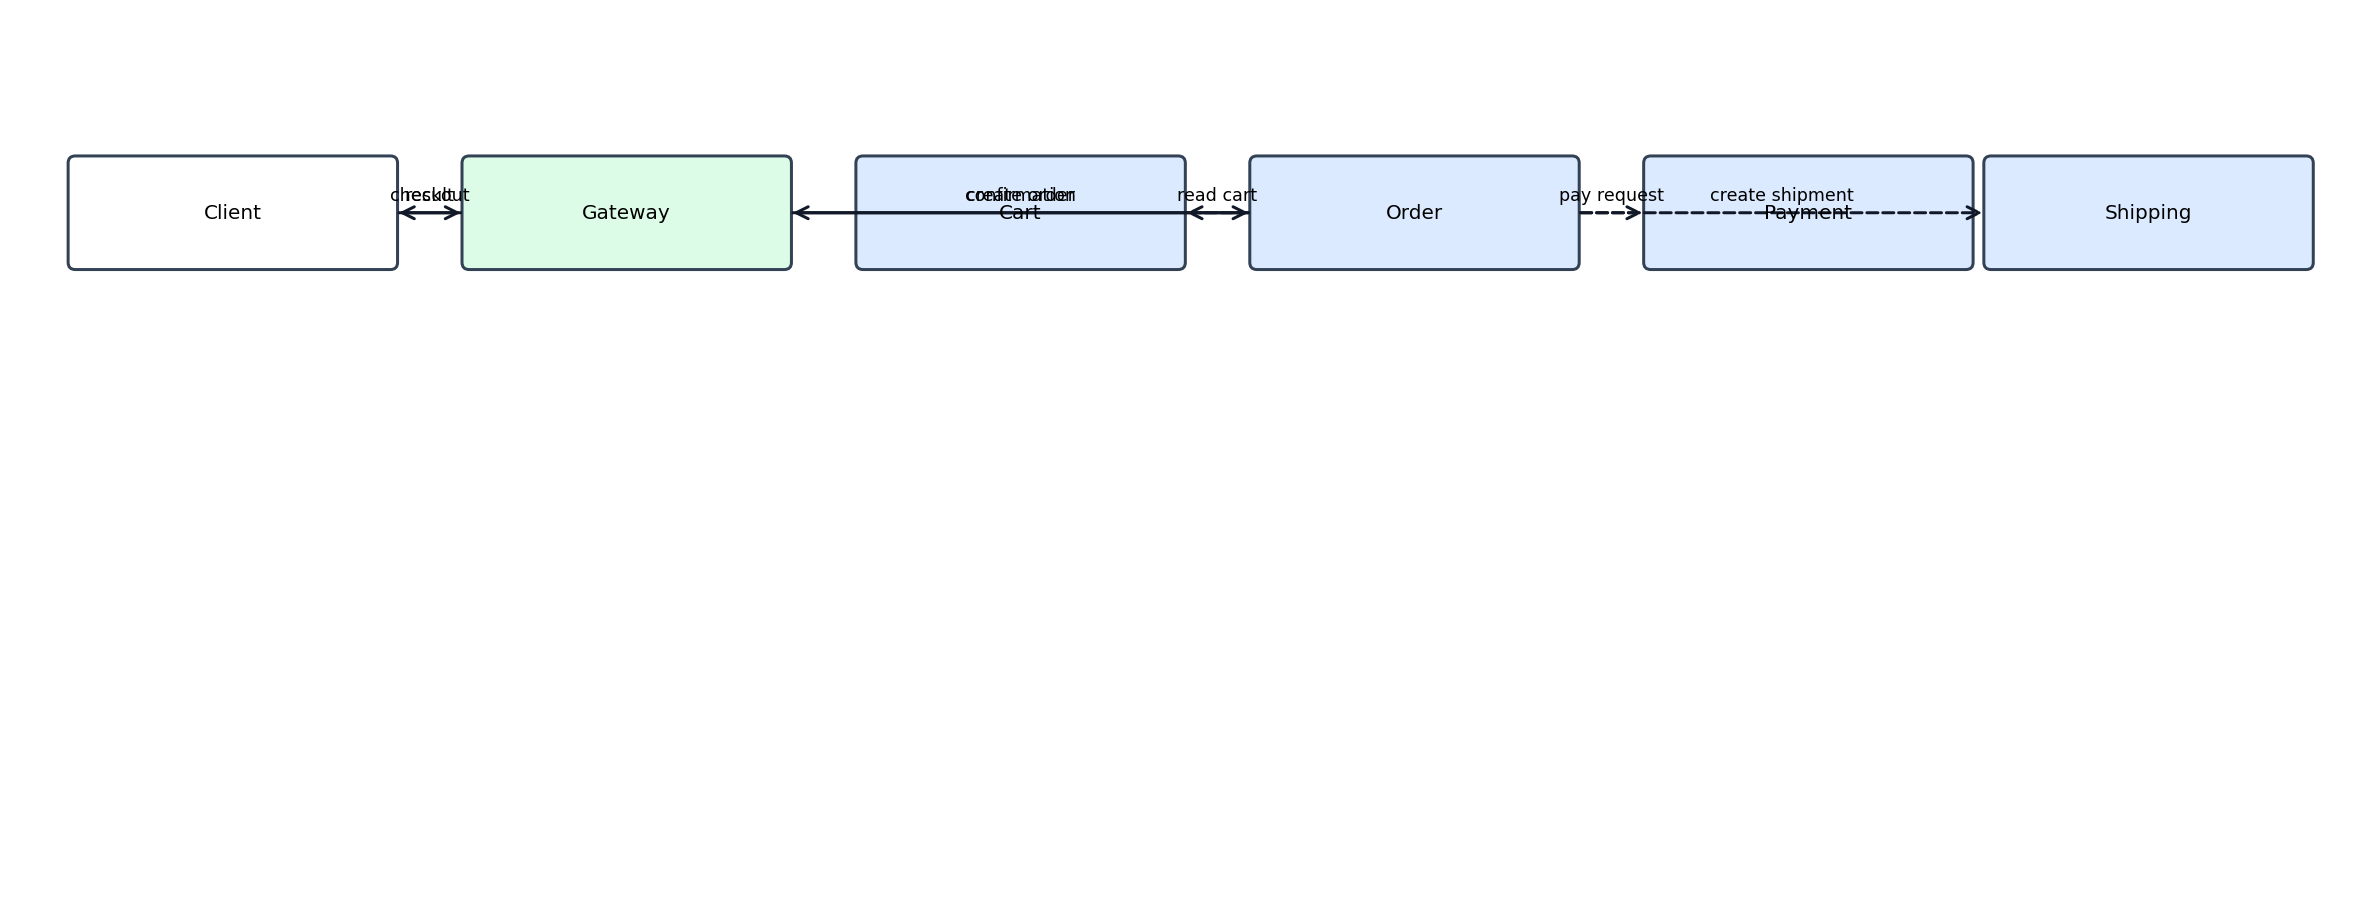
\includegraphics[width=0.98\linewidth]{generated_diagrams/ecom_checkout_sequence.png}
\caption{End-to-end checkout sequence for the e-commerce system.}
\label{fig:ecom-checkout-sequence}
\end{figure}

\subsection{Kubernetes Deployment (Optional)}

\subsubsection{Deployment}

\begin{lstlisting}[caption={Kubernetes deployment example.}]
apiVersion: apps/v1
kind: Deployment
metadata:
  name: user-service
\end{lstlisting}

\subsubsection{Service}

\begin{lstlisting}[caption={Kubernetes service example.}]
kind: Service
spec:
  type: ClusterIP
\end{lstlisting}

\subsection{Logging and Monitoring}

Logging can be implemented using the ELK stack. Monitoring can be implemented with Prometheus and Grafana. For a final production-style version, distributed tracing should be added to follow requests across gateway, order, payment, and shipping services.

\subsection{System Evaluation}

\subsubsection{Performance}

Performance can be evaluated by response time, throughput, database query time, and checkout latency.

\subsubsection{Scalability}

Each service can be scaled independently. Product-service can be scaled for browsing traffic, while payment-service can be protected more strictly.

\subsubsection{Advantages}

\begin{itemize}
    \item Flexible service evolution.
    \item Clear service ownership.
    \item Better scalability.
    \item Better alignment with DDD.
\end{itemize}

\subsubsection{Disadvantages}

\begin{itemize}
    \item More deployment complexity.
    \item More difficult debugging.
    \item More complex data consistency.
    \item Requires stronger monitoring and DevOps practice.
\end{itemize}

\subsection{Practical Exercise}

The practical part should implement Django services, connect them through APIs, dockerize the system, and test the full shopping flow with AI consultation output.

\subsection{Evaluation Checklist}

\begin{itemize}
    \item API Gateway exists.
    \item JWT authentication exists.
    \item Docker can run the system.
    \item Order to payment to shipping flow works.
    \item AI recommendation or chatbot API works.
    \item Class diagram, data model, database mapping, and architecture diagrams are included.
\end{itemize}

\section*{Final Conclusion}
\addcontentsline{toc}{section}{Final Conclusion}

This essay follows the lecturer's structure: it first explains monolithic architecture, microservices, and DDD; then it develops the main e-commerce microservice design; then it presents the AI service for product consultation; and finally it describes the complete system architecture, gateway, security, communication, Docker deployment, workflow, and evaluation.

The healthcare system appears only as the case study in Section 1.4 for practicing DDD decomposition. The main project remains the e-commerce microservices system with AI recommendation and chatbot consultation.

\section*{References}
\addcontentsline{toc}{section}{References}

\begin{enumerate}[label={[\arabic*]}]
    \item E. Evans, \textit{Domain-Driven Design: Tackling Complexity in the Heart of Software}. Addison-Wesley, 2003.
    \item S. Newman, \textit{Building Microservices: Designing Fine-Grained Systems}, 2nd ed. O'Reilly Media, 2021.
    \item M. Fowler and J. Lewis, ``Microservices: a definition of this new architectural term,'' 2014.
    \item C. Richardson, \textit{Microservices Patterns}. Manning Publications, 2018.
    \item Django Software Foundation, ``Django Documentation.'' Official documentation.
    \item Django REST Framework, ``Django REST Framework Documentation.'' Official documentation.
    \item Neo4j, ``Neo4j Graph Database Documentation.'' Official documentation.
    \item scikit-learn developers, ``scikit-learn Documentation.'' Official documentation.
\end{enumerate}

\appendix

\section{Remaining Implementation Evidence to Add Later}

Because the general e-commerce project is stored outside the current workspace, the final pass should replace generic design examples with code evidence from that project:

\begin{itemize}
    \item Real repository folder structure.
    \item Actual service names and ports.
    \item Actual models and serializers.
    \item Actual API Gateway configuration.
    \item Actual Docker Compose file.
    \item Actual database engines and schema.
    \item Screenshots or command output proving the end-to-end flow.
\end{itemize}

\end{document}
